\documentclass{standalone}
\usepackage{tikz}
\usetikzlibrary{patterns, positioning}


\begin{document}
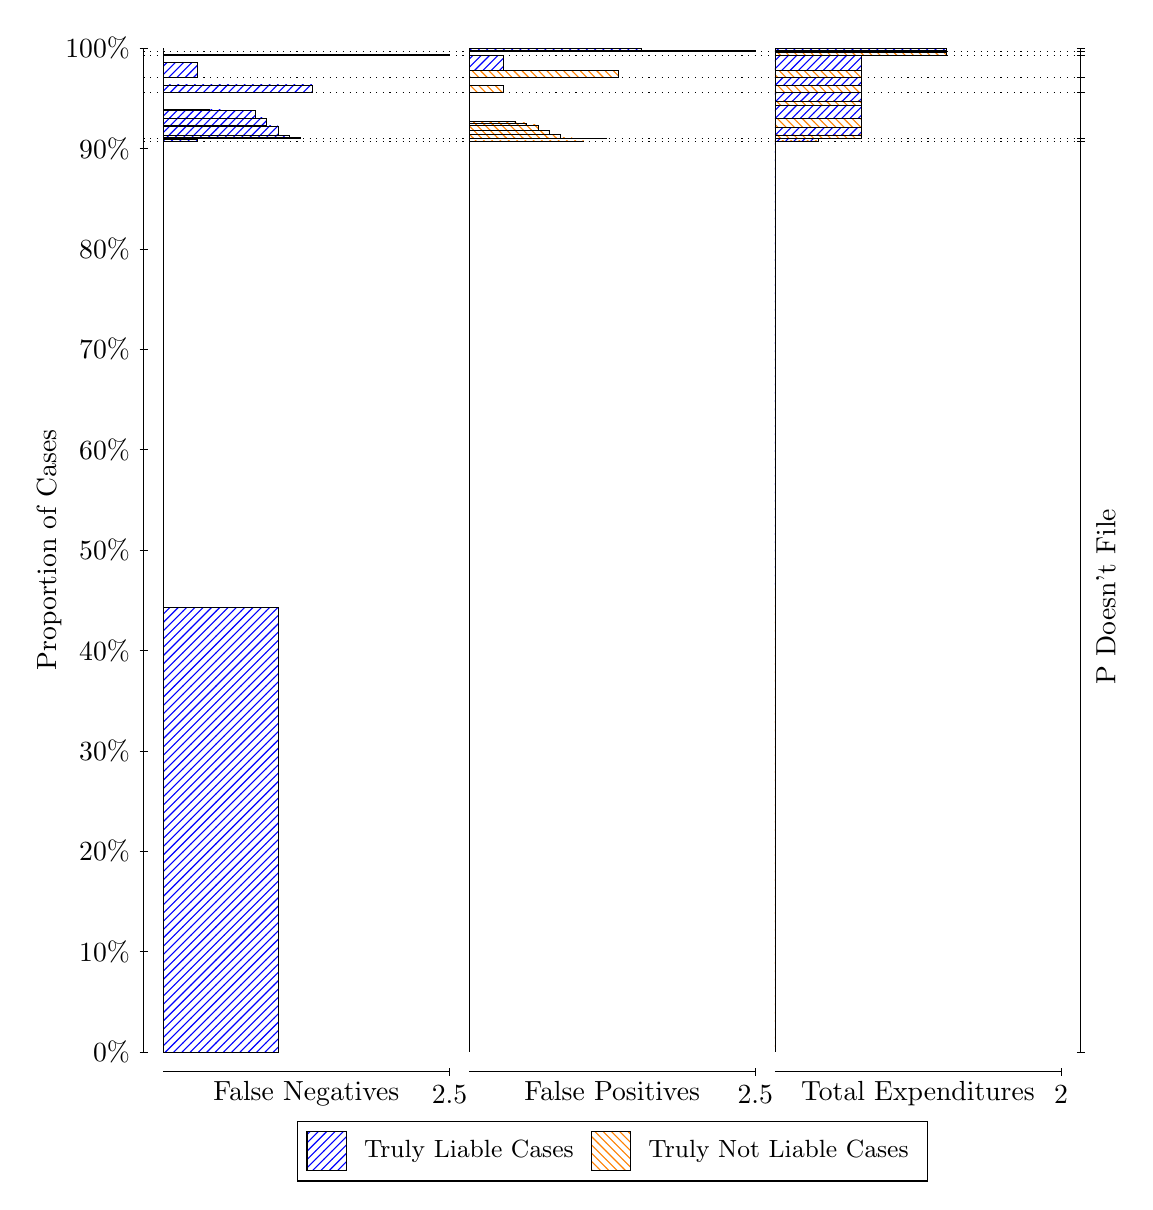
\begin{tikzpicture}
\draw[black, very thin] (1.5,1.75) -- (1.5,14.5);
\node[rotate=90, text=black, anchor=center] at (0.3, 8.125) {Proportion of Cases};
\draw[black, very thin] (1.45,1.75) -- (1.55,1.75);
\node[text=black, anchor=east] at (1.45, 1.75) {0\%};
\draw[black, very thin] (1.45,3.025) -- (1.55,3.025);
\node[text=black, anchor=east] at (1.45, 3.025) {10\%};
\draw[black, very thin] (1.45,4.3) -- (1.55,4.3);
\node[text=black, anchor=east] at (1.45, 4.3) {20\%};
\draw[black, very thin] (1.45,5.575) -- (1.55,5.575);
\node[text=black, anchor=east] at (1.45, 5.575) {30\%};
\draw[black, very thin] (1.45,6.85) -- (1.55,6.85);
\node[text=black, anchor=east] at (1.45, 6.85) {40\%};
\draw[black, very thin] (1.45,8.125) -- (1.55,8.125);
\node[text=black, anchor=east] at (1.45, 8.125) {50\%};
\draw[black, very thin] (1.45,9.4) -- (1.55,9.4);
\node[text=black, anchor=east] at (1.45, 9.4) {60\%};
\draw[black, very thin] (1.45,10.675) -- (1.55,10.675);
\node[text=black, anchor=east] at (1.45, 10.675) {70\%};
\draw[black, very thin] (1.45,11.95) -- (1.55,11.95);
\node[text=black, anchor=east] at (1.45, 11.95) {80\%};
\draw[black, very thin] (1.45,13.225) -- (1.55,13.225);
\node[text=black, anchor=east] at (1.45, 13.225) {90\%};
\draw[black, very thin] (1.45,14.5) -- (1.55,14.5);
\node[text=black, anchor=east] at (1.45, 14.5) {100\%};

\draw[black, very thin] (13.4,1.75) -- (13.4,14.5);
\draw[black, very thin] (13.35,1.75) -- (13.45,1.75);
\node[anchor=west] at (13.35, 1.75) {};
\draw[black, very thin] (13.35,13.316) -- (13.45,13.316);
\node[anchor=west] at (13.35, 13.316) {};
\draw[black, very thin] (13.35,13.35) -- (13.45,13.35);
\node[anchor=west] at (13.35, 13.35) {};
\draw[black, very thin] (13.35,13.934) -- (13.45,13.934);
\node[anchor=west] at (13.35, 13.934) {};
\draw[black, very thin] (13.35,14.128) -- (13.45,14.128);
\node[anchor=west] at (13.35, 14.128) {};
\draw[black, very thin] (13.35,14.407) -- (13.45,14.407);
\node[anchor=west] at (13.35, 14.407) {};
\draw[black, very thin] (13.35,14.46) -- (13.45,14.46);
\node[anchor=west] at (13.35, 14.46) {};
\draw[black, very thin] (13.35,14.5) -- (13.45,14.5);
\node[anchor=west] at (13.35, 14.5) {};

\draw[black, very thin, pattern color=blue, pattern=north east lines] (1.75,1.75) rectangle (3.2033,7.3995);
\draw[black, very thin, pattern color=orange, pattern=north west lines] (1.75,7.3995) rectangle (1.75,13.316);
\draw[black, very thin, pattern color=blue, pattern=north east lines] (1.75,13.316) rectangle (2.186,13.346);
\draw[black, very thin, pattern color=orange, pattern=north west lines] (1.75,13.346) rectangle (1.75,13.35);
\draw[black, very thin, pattern color=blue, pattern=north east lines] (1.75,13.35) rectangle (3.494,13.362);
\draw[black, very thin, pattern color=blue, pattern=north east lines] (1.75,13.362) rectangle (3.3487,13.393);
\draw[black, very thin, pattern color=blue, pattern=north east lines] (1.75,13.393) rectangle (3.2033,13.512);
\draw[black, very thin, pattern color=blue, pattern=north east lines] (1.75,13.512) rectangle (3.058,13.514);
\draw[black, very thin, pattern color=blue, pattern=north east lines] (1.75,13.514) rectangle (3.058,13.614);
\draw[black, very thin, pattern color=blue, pattern=north east lines] (1.75,13.614) rectangle (2.9127,13.705);
\draw[black, very thin, pattern color=blue, pattern=north east lines] (1.75,13.705) rectangle (2.7673,13.709);
\draw[black, very thin, pattern color=blue, pattern=north east lines] (1.75,13.709) rectangle (2.622,13.712);
\draw[black, very thin, pattern color=blue, pattern=north east lines] (1.75,13.712) rectangle (2.4767,13.714);
\draw[black, very thin, pattern color=blue, pattern=north east lines] (1.75,13.714) rectangle (2.3313,13.716);
\draw[black, very thin, pattern color=orange, pattern=north west lines] (1.75,13.716) rectangle (1.75,13.934);
\draw[black, very thin, pattern color=blue, pattern=north east lines] (1.75,13.934) rectangle (3.6393,14.033);
\draw[black, very thin, pattern color=orange, pattern=north west lines] (1.75,14.033) rectangle (1.75,14.128);
\draw[black, very thin, pattern color=blue, pattern=north east lines] (1.75,14.128) rectangle (2.186,14.318);
\draw[black, very thin, pattern color=orange, pattern=north west lines] (1.75,14.318) rectangle (1.75,14.407);
\draw[black, very thin, pattern color=blue, pattern=north east lines] (1.75,14.407) rectangle (5.3833,14.416);
\draw[black, very thin, pattern color=orange, pattern=north west lines] (1.75,14.416) rectangle (1.75,14.46);
\draw[black, very thin, pattern color=orange, pattern=north west lines] (1.75,14.46) rectangle (1.75,14.469);
\draw[black, very thin, pattern color=blue, pattern=north east lines] (1.75,14.469) rectangle (1.75,14.5);
\draw[black, very thin, pattern color=orange, pattern=north west lines] (5.6333,1.75) rectangle (5.6333,7.6664);
\draw[black, very thin, pattern color=blue, pattern=north east lines] (5.6333,7.6664) rectangle (5.6333,13.316);
\draw[black, very thin, pattern color=orange, pattern=north west lines] (5.6333,13.316) rectangle (7.0867,13.32);
\draw[black, very thin, pattern color=blue, pattern=north east lines] (5.6333,13.32) rectangle (5.6333,13.35);
\draw[black, very thin, pattern color=orange, pattern=north west lines] (5.6333,13.35) rectangle (7.3773,13.351);
\draw[black, very thin, pattern color=orange, pattern=north west lines] (5.6333,13.351) rectangle (7.232,13.352);
\draw[black, very thin, pattern color=orange, pattern=north west lines] (5.6333,13.352) rectangle (7.0867,13.355);
\draw[black, very thin, pattern color=orange, pattern=north west lines] (5.6333,13.355) rectangle (6.9413,13.358);
\draw[black, very thin, pattern color=orange, pattern=north west lines] (5.6333,13.358) rectangle (6.796,13.401);
\draw[black, very thin, pattern color=orange, pattern=north west lines] (5.6333,13.401) rectangle (6.6507,13.452);
\draw[black, very thin, pattern color=orange, pattern=north west lines] (5.6333,13.452) rectangle (6.5053,13.524);
\draw[black, very thin, pattern color=orange, pattern=north west lines] (5.6333,13.524) rectangle (6.36,13.549);
\draw[black, very thin, pattern color=orange, pattern=north west lines] (5.6333,13.549) rectangle (6.2147,13.568);
\draw[black, very thin, pattern color=blue, pattern=north east lines] (5.6333,13.568) rectangle (5.924,13.57);
\draw[black, very thin, pattern color=blue, pattern=north east lines] (5.6333,13.57) rectangle (5.7787,13.571);
\draw[black, very thin, pattern color=blue, pattern=north east lines] (5.6333,13.571) rectangle (5.6333,13.934);
\draw[black, very thin, pattern color=orange, pattern=north west lines] (5.6333,13.934) rectangle (6.0693,14.029);
\draw[black, very thin, pattern color=blue, pattern=north east lines] (5.6333,14.029) rectangle (5.6333,14.128);
\draw[black, very thin, pattern color=orange, pattern=north west lines] (5.6333,14.128) rectangle (7.5227,14.217);
\draw[black, very thin, pattern color=blue, pattern=north east lines] (5.6333,14.217) rectangle (6.0693,14.407);
\draw[black, very thin, pattern color=orange, pattern=north west lines] (5.6333,14.407) rectangle (5.6333,14.45);
\draw[black, very thin, pattern color=blue, pattern=north east lines] (5.6333,14.45) rectangle (5.6333,14.46);
\draw[black, very thin, pattern color=orange, pattern=north west lines] (5.6333,14.46) rectangle (9.2667,14.469);
\draw[black, very thin, pattern color=blue, pattern=north east lines] (5.6333,14.469) rectangle (7.8133,14.5);
\draw[black, very thin, pattern color=orange, pattern=north west lines] (9.5167,1.75) rectangle (9.5167,7.6664);
\draw[black, very thin, pattern color=blue, pattern=north east lines] (9.5167,7.6664) rectangle (9.5167,13.316);
\draw[black, very thin, pattern color=orange, pattern=north west lines] (9.5167,13.316) rectangle (10.062,13.32);
\draw[black, very thin, pattern color=blue, pattern=north east lines] (9.5167,13.32) rectangle (10.062,13.35);
\draw[black, very thin, pattern color=orange, pattern=north west lines] (9.5167,13.35) rectangle (10.607,13.396);
\draw[black, very thin, pattern color=blue, pattern=north east lines] (9.5167,13.396) rectangle (10.607,13.493);
\draw[black, very thin, pattern color=orange, pattern=north west lines] (9.5167,13.493) rectangle (10.607,13.61);
\draw[black, very thin, pattern color=blue, pattern=north east lines] (9.5167,13.61) rectangle (10.607,13.774);
\draw[black, very thin, pattern color=orange, pattern=north west lines] (9.5167,13.774) rectangle (10.607,13.828);
\draw[black, very thin, pattern color=blue, pattern=north east lines] (9.5167,13.828) rectangle (10.607,13.934);
\draw[black, very thin, pattern color=orange, pattern=north west lines] (9.5167,13.934) rectangle (10.607,14.029);
\draw[black, very thin, pattern color=blue, pattern=north east lines] (9.5167,14.029) rectangle (10.607,14.128);
\draw[black, very thin, pattern color=orange, pattern=north west lines] (9.5167,14.128) rectangle (10.607,14.217);
\draw[black, very thin, pattern color=blue, pattern=north east lines] (9.5167,14.217) rectangle (10.607,14.407);
\draw[black, very thin, pattern color=orange, pattern=north west lines] (9.5167,14.407) rectangle (11.697,14.45);
\draw[black, very thin, pattern color=blue, pattern=north east lines] (9.5167,14.45) rectangle (11.697,14.46);
\draw[black, very thin, pattern color=orange, pattern=north west lines] (9.5167,14.46) rectangle (11.697,14.469);
\draw[black, very thin, pattern color=blue, pattern=north east lines] (9.5167,14.469) rectangle (11.697,14.5);
\draw[black, dotted] (1.5,13.316) -- (13.4,13.316);
\draw[black, dotted] (1.5,13.35) -- (13.4,13.35);
\draw[black, dotted] (1.5,13.934) -- (13.4,13.934);
\draw[black, dotted] (1.5,14.128) -- (13.4,14.128);
\draw[black, dotted] (1.5,14.407) -- (13.4,14.407);
\draw[black, dotted] (1.5,14.46) -- (13.4,14.46);
\draw[black, very thin] (1.75,1.5) -- (5.3833,1.5);
\node[text=black, anchor=north] at (3.5667, 1.5) {False Negatives};
\draw[black, very thin] (5.3833,1.45) -- (5.3833,1.55);
\node[text=black, anchor=north] at (5.3833, 1.45) {2.5};

\draw[black, very thin] (5.6333,1.5) -- (9.2667,1.5);
\node[text=black, anchor=north] at (7.45, 1.5) {False Positives};
\draw[black, very thin] (9.2667,1.45) -- (9.2667,1.55);
\node[text=black, anchor=north] at (9.2667, 1.45) {2.5};

\draw[black, very thin] (9.5167,1.5) -- (13.15,1.5);
\node[text=black, anchor=north] at (11.333, 1.5) {Total Expenditures};
\draw[black, very thin] (13.15,1.45) -- (13.15,1.55);
\node[text=black, anchor=north] at (13.15, 1.45) {2};

\node[text=black, centered, rotate=90] at (13.72, 7.533) {P Doesn't File};







\draw (7.449999999999999,1.5) node[draw=none] (baseCoordinate) {};
\begin{scope}[align=center]
        \matrix[scale=0.5, draw=black, below=0.5cm of baseCoordinate, nodes={draw}, column sep=0.1cm]{
            \node[rectangle, draw, minimum width=0.5cm, minimum height=0.5cm, pattern color=blue, pattern=north east lines] {}; &
            \node[draw=none, font=\small, text=black] (B) {Truly Liable Cases}; &
            \node[rectangle, draw, minimum width=0.5cm, minimum height=0.5cm, pattern color=orange, pattern=north west lines] {}; &
            \node[draw=none, font=\small, text=black] (B) {Truly Not Liable Cases}; \\
            };
\end{scope}

\end{tikzpicture}
\end{document}